\documentclass[handout]{beamer}
\usetheme{metropolis}
\beamertemplatetransparentcoveredhigh

\usepackage[portuges]{babel}
\usepackage{graphicx}
\graphicspath{{./figs/}}
\usepackage{listings}
\usepackage{color}
\usepackage{hyperref}
\usepackage{xpatch}
\usepackage{comment}
\usepackage[outputdir=build]{minted}

\makeatletter
\AtBeginEnvironment{minted}{\dontdofcolorbox}
\def\dontdofcolorbox{\renewcommand\fcolorbox[4][]{##4}}
\xpatchcmd{\inputminted}{\minted@fvset}{\minted@fvset\dontdofcolorbox}{}{}
\xpatchcmd{\mintinline}{\minted@fvset}{\minted@fvset\dontdofcolorbox}{}{}
\makeatother
\setminted[c]{
  linenos=true,
  breaklines=true,
  encoding=utf8,
  frame=lines,
  framerule=0.5pt,
  autogobble,
  fontsize=\small,
}
\setminted[bash]{
  linenos=true,
  encoding=utf8,
  frame=lines,
  framerule=0.5pt,
  autogobble,
  fontsize=\small
}

\newcommand{\cod}[1]{\mintinline{c}{#1}}


\definecolor{dkgreen}{rgb}{0,0.6,0}
\definecolor{gray}{rgb}{0.5,0.5,0.5}
\definecolor{mauve}{rgb}{0.58,0,0.82}


\definecolor{Purple}{HTML}{911146}
\definecolor{Orange}{HTML}{CF4A30}
\setbeamercolor{alerted text}{fg=Orange}
\setbeamercolor{frametitle}{bg=Purple}
\setbeamercolor{block body}{bg=Purple!20,fg=black}
\setbeamercolor{block title}{bg=Purple!50,fg=black}
\setbeamertemplate{blocks}[rounded][shadow=true]


\newcounter{ExercicioCounter}
\newcommand{\exercicio}{\refstepcounter{ExercicioCounter} Exercício~\theExercicioCounter}

\newcommand{\setcoverbg}{
  \setbeamertemplate{background}
  {
\includegraphics[width=\paperwidth,height=\paperheight]{backgrounds/coverbg}}
}
\newcommand{\setsectionbg}{
  \setbeamertemplate{background}
  {
\includegraphics[width=\paperwidth,height=\paperheight]{backgrounds/blank}}
}

\title{Programação Estruturada}
\subtitle{Vetores e matrizes}

\author{Professores Emílio Francesquini e Carla Negri Lintzmayer}
\institute{Centro de Matemática, Computação e Cognição\\ Universidade Federal do ABC}
\date{2018.Q3}

\begin{document}

\setcoverbg
\maketitle
\setsectionbg




%%%%%%%%%%%%%%%%%%%%%%%%%%%%%%%%%%%%%%%%%%%%%%%%%%%
%%%%%%%%%%%%%%%%%%%%%%%%%%%%%%%%%%%%%%%%%%%%%%%%%%%
%%%%%%%%%%%%%%%%%%%%%%%%%%%%%%%%%%%%%%%%%%%%%%%%%%%
%%%%%%%%%%%%%%%%%%%%%%%%%%%%%%%%%%%%%%%%%%%%%%%%%%%
%%%%%%%%%%%%%%%%%%%%%%%%%%%%%%%%%%%%%%%%%%%%%%%%%%%
%%%%%%%%%%%%%%%%%%%%%%%%%%%%%%%%%%%%%%%%%%%%%%%%%%%

\section{Introdução}

%%%%%%%%%%%%%%%%%%%%%%%%%%%%%%%%%%%%%%%%%%%%%%%%
\begin{frame}[fragile]{Motivação}

    Suponha que desejamos guardar notas de alunos.

    Com o que aprendemos até agora, como armazenaríamos 3 notas?

    \begin{minted}{c}
        float nota1, nota2, nota3;

        printf("Nota do aluno 1: ");
        scanf("%f", &nota1);
        printf("Nota do aluno 2: ");
        scanf("%f", &nota2);
        printf("Nota do aluno 3: ");
        scanf("%f", &nota3);
    \end{minted}

\end{frame}

%%%%%%%%%%%%%%%%%%%%%%%%%%%%%%%%%%%%%%%%%%%%%%%%%%%
\begin{frame}[fragile]{Motivação}

    Com o que sabemos, como armazenaríamos 100 notas?

    \begin{minted}{c}
        float nota1, nota2, nota3,..., nota100;

        printf("Nota do aluno 1: ");
        scanf("%f", &nota1);
        printf("Nota do aluno 2: ");
        scanf("%f", &nota2);
        ...
        printf("Nota do aluno 100: ");
        scanf("%f", &nota100);
    \end{minted}

    Apesar de ainda ser viável, criar 100 variáveis distintas não é uma solução elegante para este problema.
    E se precisássemos armazenar 1.000.000 notas? Ou $n$ notas?

\end{frame}

%%%%%%%%%%%%%%%%%%%%%%%%%%%%%%%%%%%%%%%%%%%%%%%%%%%
%%%%%%%%%%%%%%%%%%%%%%%%%%%%%%%%%%%%%%%%%%%%%%%%%%%
%%%%%%%%%%%%%%%%%%%%%%%%%%%%%%%%%%%%%%%%%%%%%%%%%%%
%%%%%%%%%%%%%%%%%%%%%%%%%%%%%%%%%%%%%%%%%%%%%%%%%%%
%%%%%%%%%%%%%%%%%%%%%%%%%%%%%%%%%%%%%%%%%%%%%%%%%%%
%%%%%%%%%%%%%%%%%%%%%%%%%%%%%%%%%%%%%%%%%%%%%%%%%%%

\section{Vetores}

%%%%%%%%%%%%%%%%%%%%%%%%%%%%%%%%%%%%%%%%%%%%%%%%%%%
%%%%%%%%%%%%%%%%%%%%%%%%%%%%%%%%%%%%%%%%%%%%%%%%%%%
%%%%%%%%%%%%%%%%%%%%%%%%%%%%%%%%%%%%%%%%%%%%%%%%%%%

\subsection{Definição de vetores}

%%%%%%%%%%%%%%%%%%%%%%%%%%%%%%%%%%%%%%%%%%%%%%%%%%%
\begin{frame}{Definição de vetores}

    \begin{itemize}[<+->]
        \item Um vetor em C é uma coleção de variáveis de um mesmo tipo que são referenciadas por um {\bf identificador único}.
        \item Características de um vetor:
        \begin{itemize}
            \item As variáveis ocupam posições contíguas na memória.
            \item O acesso se dá por meio de um índice inteiro.
            \item O vetor possui um tamanho pré-definido.
            \item O acesso do vetor com um índice fora dos limites pode causar comportamento anômalo do programa.
        \end{itemize}
    \end{itemize}

\end{frame}

%%%%%%%%%%%%%%%%%%%%%%%%%%%%%%%%%%%%%%%%%%%%%%%%%%%
\begin{frame}[fragile]{Declaração de um vetor}

    Para declarar um vetor usamos a seguinte sintaxe:
    \begin{minted}{c}
        tipo identificador[tamanho];
    \end{minted}

    Exemplos:
    \begin{minted}{c}
        /* vetor "notas" equivale a 100 variáveis do tipo float */
        float notas[100];

        /* vetor "primos" equivale a 20 variáveis do tipo int */
        int primos[20];
    \end{minted}

\end{frame}

%%%%%%%%%%%%%%%%%%%%%%%%%%%%%%%%%%%%%%%%%%%%%%%%%%%
%%%%%%%%%%%%%%%%%%%%%%%%%%%%%%%%%%%%%%%%%%%%%%%%%%%
%%%%%%%%%%%%%%%%%%%%%%%%%%%%%%%%%%%%%%%%%%%%%%%%%%%

\subsection{Vetores -- Como usar}

%%%%%%%%%%%%%%%%%%%%%%%%%%%%%%%%%%%%%%%%%%%%%%%%%%%
\begin{frame}[fragile]{Usando um vetor}

    \begin{itemize}[<+->]
        \item Após declarada uma variável do tipo vetor, pode-se acessar uma determinada posição utilizando-se um índice de valor inteiro.
        \item Sendo $n$ o tamanho do vetor, os índices válidos para o vetor vão de $0$ até $n-1$.
        \begin{itemize}
            \item A primeira posição de um vetor tem índice 0.
            \item A última posição de um vetor tem índice $n-1$.
            \item A $i$-ésima posição tem índice $i-1$.
            \item A sintaxe para acesso de uma determinada posição é:
            \cod{identificador[posicao]}
            \begin{itemize}
                \item Lê-se \cod{vet[4]} como ``vetor \cod{vet} na posição 4''
                \item \cod{vet[4]} é o quinto elemento do vetor \cod{vet}
            \end{itemize}
        \end{itemize}
    \end{itemize}

\end{frame}

%%%%%%%%%%%%%%%%%%%%%%%%%%%%%%%%%%%%%%%%%%%%%%%%%%%
\begin{frame}[fragile]{Usando um vetor}

    Uma posição específica de um vetor tem o mesmo comportamento que uma variável simples.

    \begin{minted}{c}
        int nota[10];
        int a;
        /* "nota[5]" corresponde a uma variável inteira */
        nota[5] = 95;
        a = nota[5];
    \end{minted}

\end{frame}

%%%%%%%%%%%%%%%%%%%%%%%%%%%%%%%%%%%%%%%%%%%%%%%%%%%
\begin{frame}[fragile]{Usando um vetor}

    \begin{itemize}
        \item Você deve usar apenas valores inteiros como índice para acessar uma posição do vetor.
        \item O valor pode ser inclusive uma outra variável inteira. 
    \end{itemize}

    \begin{minted}{c}
        int g, vet[10];
        for(g = 0; g < 10; g++)
            vet[g] = 5 * g;
    \end{minted}

    Quais valores estarão armazenados em cada posição do vetor após a execução deste código?

\end{frame}

%%%%%%%%%%%%%%%%%%%%%%%%%%%%%%%%%%%%%%%%%%%%%%%%%%%
%%%%%%%%%%%%%%%%%%%%%%%%%%%%%%%%%%%%%%%%%%%%%%%%%%%
%%%%%%%%%%%%%%%%%%%%%%%%%%%%%%%%%%%%%%%%%%%%%%%%%%%

\subsection{Vetores e a memória}

%%%%%%%%%%%%%%%%%%%%%%%%%%%%%%%%%%%%%%%%%%%%%%%%%%%
\begin{frame}[fragile]{Vetores e a memória}

    Suponha o código:
    \begin{minted}{c}
        int d;
        int vetor[5];
        int f;
    \end{minted}

    Na memória temos:
    \begin{center}
        \begin{tabular}{|c|c|c|c|c|c|c|c|}
          \hline
          Nome & \cod{d} & \multicolumn{5}{|c|}{\cod{vetor}} & \cod{f} \\
          \hline
          Índice & - & 0 & 1 & 2 & 3 & 4 & - \\
          \hline
               & & & & & & & \\
          \hline
        \end{tabular}
    \end{center}

\end{frame}

%%%%%%%%%%%%%%%%%%%%%%%%%%%%%%%%%%%%%%%%%%%%%%%%%%%
\begin{frame}[fragile]{Vetores e a memória}

    Ao executar o comando
    \begin{minted}{c}
        vetor[3] = 10;
    \end{minted}

    Temos em memória:

    \begin{center}
        \begin{tabular}{|c|c|c|c|c|c|c|c|}
          \hline
          Nome & \cod{d} & \multicolumn{5}{|c|}{\cod{vetor}} & \cod{f} \\
          \hline
          Índice & - & 0 & 1 & 2 & 3 & 4 & - \\
          \hline
               & & & & & 10 & & \\
          \hline
        \end{tabular}
    \end{center}

\end{frame}

%%%%%%%%%%%%%%%%%%%%%%%%%%%%%%%%%%%%%%%%%%%%%%%%%%%
\begin{frame}[fragile]{Vetores e a memória}

    \small
    E ao executar os comandos a seguir?
    \begin{minted}{c}
        vetor[3] = 10;
        vetor[5] = 5;
        vetor[-1] = 1;
    \end{minted}

    Teremos em memória:

    \begin{center}
        \begin{tabular}{|c|c|c|c|c|c|c|c|}
          \hline
          Nome & \cod{d} & \multicolumn{5}{|c|}{\cod{vetor}} & \cod{f} \\
          \hline
          Índice & - & 0 & 1 & 2 & 3 & 4 & - \\
          \hline
               & 1 & & & & 10 & & 5 \\
          \hline
        \end{tabular}
    \end{center}

    Seu programa estará errado pois você está alterando inadvertidamente valores de outras variáveis.

    Ele será encerrado ({\bf Segmentation Fault}) ou poderá continuar executando, mas ocorrerão erros difíceis de serem rastreados.

\end{frame}

%%%%%%%%%%%%%%%%%%%%%%%%%%%%%%%%%%%%%%%%%%%%%%%%%%%
\begin{frame}{Questões importantes sobre vetores}

    \begin{itemize}
        \item O tamanho do vetor é pré-definido (durante a execução do programa não pode ser alterado).
        \item O uso de índices fora dos limites pode causar comportamento anômalo do programa.
    \end{itemize}

\end{frame}

%%%%%%%%%%%%%%%%%%%%%%%%%%%%%%%%%%%%%%%%%%%%%%%%%%%
\begin{frame}[fragile]{Como armazenar até 100 notas?}

    \begin{minted}{c}
        float nota[100];
        int n, i;

        printf("Número de alunos: ");
        scanf("%d", &n);

        for (i = 0; i < n; i++) {
            printf("Digite a nota do aluno %d: ", i);
            scanf("%f", &nota[i]);
        }
    \end{minted}

    O programa acima está correto?

\end{frame}

%%%%%%%%%%%%%%%%%%%%%%%%%%%%%%%%%%%%%%%%%%%%%%%%%%%
\begin{frame}[fragile]{Como armazenar até 100 notas?}

    Você deve testar se $n>100$ para evitar erros!!

    \begin{minted}[fontsize=\footnotesize]{c}
        float nota[100];
        int n, i;

        printf("Número de alunos: ");
        scanf("%d", &n);

        if (n > 100) {
            n = 100;
            printf("Numero maximo de alunos alterado para 100\n");
        }

        for (i = 0; i < n; i++) {
            printf("Digite a nota do aluno %d: ", i);
            scanf("%f", &nota[i]);
        }
    \end{minted}

\end{frame}

%%%%%%%%%%%%%%%%%%%%%%%%%%%%%%%%%%%%%%%%%%%%%%%%%%%
%%%%%%%%%%%%%%%%%%%%%%%%%%%%%%%%%%%%%%%%%%%%%%%%%%%
%%%%%%%%%%%%%%%%%%%%%%%%%%%%%%%%%%%%%%%%%%%%%%%%%%%

\subsection{Vetores -- Exemplos}

%%%%%%%%%%%%%%%%%%%%%%%%%%%%%%%%%%%%%%%%%%%%%%%%%%%
\begin{frame}[fragile]{Exemplo: produto interno de dois vetores}

    \begin{block}{Problema}
        Ler dois vetores de dimensão 5 e computar o produto interno (produto escalar) destes.
    \end{block}

    Quais tipos de variáveis usar?

\end{frame}

%%%%%%%%%%%%%%%%%%%%%%%%%%%%%%%%%%%%%%%%%%%%%%%%%%%
\begin{frame}[fragile]{Exemplo: produto interno de dois vetores}

    Abaixo temos o código para ler dois vetores de dimensão 5.

    \begin{minted}[fontsize=\scriptsize]{c}
        int main() {
            double vetor1[5], vetor2[5], resultado;
            int i;

            for (i = 0; i < 5; i++) {
                printf("Entre com valor da posição %d para vetor 1: ", i);
                scanf("%lf", &vetor1[i]);
            }
            printf("\n\n");
            for (i = 0; i < 5; i++) {
                printf("Entre com valor da posição %d para vetor 2:", i);
                scanf("%lf", &vetor2[i]);
            }

            /* calculando o produto interno */
            ...
        }
    \end{minted}

\end{frame}

%%%%%%%%%%%%%%%%%%%%%%%%%%%%%%%%%%%%%%%%%%%%%%%%%%%
\begin{frame}[fragile]{Exemplo: produto interno de dois vetores}

    Abaixo temos a parte do código para computar o produto interno dos vetores.

    \begin{minted}[fontsize=\footnotesize]{c}
        int main() {
            double vetor1[5], vetor2[5], resultado;
            int i;

            ...

            /* calculando o produto interno */
            resultado = 0.0;
            for (i = 0; i < 5; i++) {
                resultado = resultado + (vetor1[i] * vetor2[i]);
            }
            printf("\n\nO produto interno é: %lf\n", resultado);
            return 0;
        }
    \end{minted}

\end{frame}

%%%%%%%%%%%%%%%%%%%%%%%%%%%%%%%%%%%%%%%%%%%%%%%%%%%
\begin{frame}[fragile]{Exemplo: produto interno de dois vetores -- código completo}

    \begin{minted}[fontsize=\scriptsize]{c}
        int main() {
            double vetor1[5], vetor2[5], resultado;
            int i;

            for (i = 0; i < 5; i++) {
                printf("Entre com valor da posição %d para vetor 1: ", i);
                scanf("%lf", &vetor1[i]);
            }
            printf("\n\n");
            for (i = 0; i < 5; i++) {
                printf("Entre com valor da posição %d para vetor 2: ", i);
                scanf("%lf", &vetor2[i]);
            }
            /* calculando o produto interno */
            resultado = 0.0;
            for (i = 0; i < 5; i++)
                resultado = resultado + (vetor1[i] * vetor2[i]);
            printf("\n\nO produto interno é: %lf\n", resultado);
            return 0;
        }
    \end{minted}

\end{frame}

%%%%%%%%%%%%%%%%%%%%%%%%%%%%%%%%%%%%%%%%%%%%%%%%%%%
\begin{frame}[fragile]{Exemplo: elementos iguais}

    \begin{itemize}
        \item Ler dois vetores com 5 inteiros cada.
        \item Checar quais elementos do segundo vetor são iguais a algum elemento do primeiro vetor.
        \item Se não houver elementos em comum, o programa deve informar isso.
    \end{itemize}

\end{frame}

%%%%%%%%%%%%%%%%%%%%%%%%%%%%%%%%%%%%%%%%%%%%%%%%%%%
\begin{frame}[fragile]{Exemplo: elementos iguais}

    Abaixo está o código que faz a leitura de dois vetores.

    \begin{minted}[fontsize=\footnotesize]{c}
        int main() {
            int vetor1[5], vetor2[5];
            int i, j, umEmComum;

            for (i = 0; i < 5; i++) {
                printf("Entre com valor da posição %d do vetor 1: ", i);
                scanf("%d", &vetor1[i]);
            }
            printf("\n\n");
            for (i = 0; i < 5; i++) {
                printf("Entre com valor da posição %d do vetor 2: ", i);
                scanf("%d", &vetor2[i]);
            }
            ...
        }
    \end{minted}

\end{frame}

%%%%%%%%%%%%%%%%%%%%%%%%%%%%%%%%%%%%%%%%%%%%%%%%%%%
\begin{frame}[fragile]{Exemplo: elementos iguais}

    \begin{itemize}
        \item Para cada elemento do \cod{vetor1} testamos todos os outros elementos do \cod{vetor2} para saber se são iguais.
        \item Usamos uma variável indicadora para decidir, ao final dos laços encaixados, se os vetores possuem ou não um elemento em comum.
    \end{itemize}

\end{frame}

%%%%%%%%%%%%%%%%%%%%%%%%%%%%%%%%%%%%%%%%%%%%%%%%%%%
\begin{frame}[fragile]{Exemplo: elementos iguais}

    \begin{minted}[fontsize=\footnotesize]{c}
        int main() {
            int vetor1[5], vetor2[5];
            int i, j, umEmComum;
            ...
            umEmComum = 0; /* Assumimos que não haja elementos comuns */
            for (i = 0; i < 5; i++) {
                for (j = 0; j < 5; j++) {
                    if (vetor1[i] == vetor2[j]) {
                        umEmComum = 1;  /* Achamos um elemento comum */
                        printf("vetor1[%d] == vetor2[%d]\n", i, j);
                    }
                }
            }
            if (!umEmComum)
                printf("Nenhum elemento em comum!\n");
            return 0;
        }
    \end{minted}

\end{frame}

%%%%%%%%%%%%%%%%%%%%%%%%%%%%%%%%%%%%%%%%%%%%%%
%%%%%%%%%%%%%%%%%%%%%%%%%%%%%%%%%%%%%%%%%%%%%%
%%%%%%%%%%%%%%%%%%%%%%%%%%%%%%%%%%%%%%%%%%%%%%

\subsection{Informações extras: inicialização de um vetor}

%%%%%%%%%%%%%%%%%%%%%%%%%%%%%%%%%%%%%%%%%%%%%%
\begin{frame}[fragile]{Informações extras: inicialização de um vetor}

    \begin{itemize}
        \item Em algumas situações é necessário declarar e já atribuir um conjunto de valores constantes para um vetor.
        \item Em C, isto é feito atribuindo-se uma lista de elementos para o vetor na sua criação da seguinte forma:

        \begin{minted}{c}
            tipo identificador[] = {elementos separados por vírgula};
        \end{minted}

        \pause

        \item Exemplos:
        \begin{minted}[fontsize=\footnotesize]{c}
            double vet1[] = {2.3, 3.4, 4.5, 5.6};
            int vet2[] = {5, 4, 3, 10, -1, 0};
        \end{minted}

        \item Note que automaticamente é criado um vetor com tamanho igual ao número de dados da inicialização.
    \end{itemize}

\end{frame}

%%%%%%%%%%%%%%%%%%%%%%%%%%%%%%%%%%%%%%%%%%%%%%
\begin{frame}[fragile]{Informações extras: inicialização de um vetor}

    \begin{minted}[fontsize=\scriptsize]{c}
        #include <stdio.h>

        int main() {
            double vet1[] = {2.3, 3.4, 4.5, 5.6};
            int vet2[] = {5, 4, 3, 10, -1, 0};
            int i;

            for (i = 0; i < 4; i++)
                printf("%lf\n", vet1[i]);

            for (i = 0; i < 6; i++)
                printf("%d\n", vet2[i]);
            
            return 0;
        }
    \end{minted}

\end{frame}

%%%%%%%%%%%%%%%%%%%%%%%%%%%%%%%%%%%%%%%%%%%%%%%%%%%
%%%%%%%%%%%%%%%%%%%%%%%%%%%%%%%%%%%%%%%%%%%%%%%%%%%
%%%%%%%%%%%%%%%%%%%%%%%%%%%%%%%%%%%%%%%%%%%%%%%%%%%
%%%%%%%%%%%%%%%%%%%%%%%%%%%%%%%%%%%%%%%%%%%%%%%%%%%
%%%%%%%%%%%%%%%%%%%%%%%%%%%%%%%%%%%%%%%%%%%%%%%%%%%
%%%%%%%%%%%%%%%%%%%%%%%%%%%%%%%%%%%%%%%%%%%%%%%%%%%

\section{Strings}

%%%%%%%%%%%%%%%%%%%%%%%%%%%%%%%%%%%%%%%%%%%%%%%%%%%
%%%%%%%%%%%%%%%%%%%%%%%%%%%%%%%%%%%%%%%%%%%%%%%%%%%
%%%%%%%%%%%%%%%%%%%%%%%%%%%%%%%%%%%%%%%%%%%%%%%%%%%

\subsection{Definição de strings em C}

%%%%%%%%%%%%%%%%%%%%%%%%%%%%%%%%%%%%%%%%%%%%%%%%%%%
\begin{frame}[fragile]{Strings em C}

    \begin{itemize}[<+->]
        \item A linguagem C não possui o tipo {\it string} explicitamente, mas podemos considerar um vetor de caracteres como uma string.
        \item Em C, uma string é sempre terminada pelo caractere `\textbackslash0'.

        \begin{block}{Definição}
            Uma string em C corresponde a um vetor de caracteres terminado pelo caractere especial `\textbackslash0'.
        \end{block}

        \item Sempre declare uma string com um caractere a mais do que precisa, já que também será preciso armazenar o `\textbackslash0'.
        \begin{itemize}
            \item Se por exemplo, estivermos trabalhando com strings de 10 caracteres, declare uma variável com tamanho 11:
            \begin{minted}[fontsize=\footnotesize]{c}
                char st[11];
            \end{minted}
        \end{itemize}
    \end{itemize}

\end{frame}

%%%%%%%%%%%%%%%%%%%%%%%%%%%%%%%%%%%%%%%%%%%%%%%%%%%
\begin{frame}[fragile]{Strings em C}

    {\bf Lembre-se:} o caractere `\textbackslash0' identifica o final da string.

    No programa abaixo gostaríamos que fosse impresso ``ola''.

    \begin{minted}[fontsize=\scriptsize]{c}
        int main() {
            char st[80];

            st[0] = 'o';
            st[1] = 'l';
            st[2] = 'a';

            printf("%s\n", st);
            return 0;
        }
    \end{minted}

    Mas às vezes será impresso uma palavra diferente, como ``ola8uj?'', pois não identificamos o final da string.

\end{frame}

%%%%%%%%%%%%%%%%%%%%%%%%%%%%%%%%%%%%%%%%%%%%%%%%%%%
\begin{frame}[fragile]{Strings em C}

    A versão correta do programa seria esta abaixo.

    \begin{minted}[fontsize=\scriptsize]{c}
        int main() {
            char st[80];

            st[0] = 'o';
            st[1] = 'l';
            st[2] = 'a';
            st[3] = '\0';

            printf("%s\n", st);
            return 0;
        }
    \end{minted}
        
    Note que a variável \cod{st} pode armazenar strings com até 79 caracteres, mas neste exemplo só estamos usando 3 (além do `\textbackslash0').

\end{frame}

%%%%%%%%%%%%%%%%%%%%%%%%%%%%%%%%%%%%%%%%%%%%%%%%%%%
%%%%%%%%%%%%%%%%%%%%%%%%%%%%%%%%%%%%%%%%%%%%%%%%%%%
%%%%%%%%%%%%%%%%%%%%%%%%%%%%%%%%%%%%%%%%%%%%%%%%%%%

\subsection{Leitura e escrita de strings}

%%%%%%%%%%%%%%%%%%%%%%%%%%%%%%%%%%%%%%%%%%%%%%%%%%%
\begin{frame}[fragile]{Leitura e escrita de strings}

    \small
    Para ler/imprimir uma string do teclado usamos o operador {\bf \%s}.

    \begin{minted}[fontsize=\scriptsize]{c}
        int main() {
            char st[80];
            int id;

            printf("Entre com o nome: ");
            scanf("%s", st);
            printf("Entre com a idade:");
            scanf("%d", &id);

            printf("Digitado: %s e %d\n", st, id);
            return 0;
        }
    \end{minted}

    Note que para strings não é utilizado o $\&$ antes do identificador da variável no comando \cod{scanf}.

    O \cod{scanf} automaticamente coloca um `\textbackslash0' ao final da string lida.

\end{frame}

%%%%%%%%%%%%%%%%%%%%%%%%%%%%%%%%%%%%%%%%%%%%%%%%%%%
\begin{frame}[fragile]{Leitura e escrita de strings}

    \small
    \cod{scanf} com \texttt{\%s} termina a leitura em uma quebra de linha ou um espaço.

    \begin{minted}[fontsize=\scriptsize]{c}
        char st[80];
        int id;
        printf("Entre com o nome: ");
        scanf("%s", st);
        printf("Entre com a idade: ");
        scanf("%d", &id);
        printf("Digitado: %s e %d\n", st, id);
    \end{minted}

    No exemplo acima, se digitarmos
    \begin{minted}[fontsize=\scriptsize]{bash}
        Joao da Silva
        19
    \end{minted}
    será salvo apenas ``Joao'' em \cod{st}, e um valor diferente de 19 em \cod{id}, porque o \cod{scanf} lê a string até o primeiro espaço, e converte o próximo dado (que é a string ``da'') em um inteiro.

\end{frame}

%%%%%%%%%%%%%%%%%%%%%%%%%%%%%%%%%%%%%%%%%%%%%%%%%%%
\begin{frame}[fragile]{Leitura e escrita de strings}

    \small
    \begin{itemize}[<+->]
        \item Para ler strings {\bf incluindo espaços} use o comando \cod{fgets}:
        \begin{minted}{c}
            fgets(identificador, limite, stdin);
        \end{minted}
        onde \cod{identificador} é o nome da variável para onde será lida a string, \cod{limite - 1} é a quantidade máxima de caracteres que poderá ser lida, e \cod{stdin} é uma palavra reservada que indica que a leitura se dará da entrada padrão.

        \item Serão lidos todos os caracteres até uma quebra de linha, e todos serão armazenados na variável \cod{identificador}, \textbf{incluindo o caractere de quebra de linha}, a menos que \cod{limite-1} caracteres tenham sido lidos, caso em que a função para a leitura antes da quebra de linha.

        \item A função inclui um `\textbackslash0' na posição final, após os caracteres lidos.
    \end{itemize}

\end{frame}

%%%%%%%%%%%%%%%%%%%%%%%%%%%%%%%%%%%%%%%%%%%%%%%%%%%
\begin{frame}[fragile]{Leitura e escrita de strings}

    \small
    \begin{minted}[fontsize=\scriptsize]{c}
         char st[80];
         int id;

         printf("Entre com o nome: ");
         fgets(st, 80, stdin);
         printf("Entre com a idade: ");
         scanf("%d", &id);
    \end{minted}

    No exemplo acima se digitarmos
    \begin{minted}[fontsize=\scriptsize]{bash}
        Joao da Silva
        19
    \end{minted}

    Será salvo ``Joao da Silva\textbackslash{n}\textbackslash{0}'' em \cod{st}, e o valor 19 em \cod{id}.

    Como \cod{st} pode armazenar até 80 caracteres, usamos este valor como parâmetro para o limite de caracteres que podem ser lidos do teclado, já que serão lidos até 79, e deve ser incluído o `\textbackslash0' no final.

\end{frame}

%%%%%%%%%%%%%%%%%%%%%%%%%%%%%%%%%%%%%%%%%%%%%%%%%%%
\begin{frame}[fragile]{Leitura e escrita de strings}

    \begin{itemize}[<+->]
        \item Em geral é mais seguro usar o \cod{fgets} do que o \cod{scanf}, pois o primeiro especifica o tamanho máximo da string a ser lida.
        \item Se um usuário digitar uma string maior do que o vetor declarado, o \cod{scanf} pode dar problemas pois irá ler todos caracteres até um espaço ou `\textbackslash n', sobrescrevendo posições inválidas da memória.
        \item Existe um ataque conhecido como {\it buffer overflow} que explora justamente este problema do \cod{scanf}.
        \item Já o \cod{fgets} sempre lê uma string de até o máximo especificado.
    \end{itemize}

\end{frame}

%%%%%%%%%%%%%%%%%%%%%%%%%%%%%%%%%%%%%%%%%%%%%%%%%%%
%%%%%%%%%%%%%%%%%%%%%%%%%%%%%%%%%%%%%%%%%%%%%%%%%%%
%%%%%%%%%%%%%%%%%%%%%%%%%%%%%%%%%%%%%%%%%%%%%%%%%%%

\subsection{Inicialização de strings}

%%%%%%%%%%%%%%%%%%%%%%%%%%%%%%%%%%%%%%%%%%%%%%%%%%%
\begin{frame}[fragile]{Inicialização de strings}

    \begin{itemize}[<+->]
        \item Em algumas situações, ao criarmos uma string, pode ser útil atribuir valores já na sua criação.
        \item No caso de strings, podemos atribuir diretamente uma constante string para a variável.

        \begin{minted}{c}
            char st[100] = "sim, isto é possível";
        \end{minted}

        \item O comando de inicialização automaticamente insere o caractere `\textbackslash{0}' no final da string.
        \item Atribuições posteriores à inicialização, no entanto, não são permitidas!
    \end{itemize}

\end{frame}

%%%%%%%%%%%%%%%%%%%%%%%%%%%%%%%%%%%%%%%%%%%%%%%%%%%
%%%%%%%%%%%%%%%%%%%%%%%%%%%%%%%%%%%%%%%%%%%%%%%%%%%
%%%%%%%%%%%%%%%%%%%%%%%%%%%%%%%%%%%%%%%%%%%%%%%%%%%

\subsection{Strings: exemplos}

%%%%%%%%%%%%%%%%%%%%%%%%%%%%%%%%%%%%%%%%%%%%%%%%%%%
\begin{frame}[fragile]{Strings: exemplos}

    \begin{block}{Problema}
        Ler uma string de até 79 caracteres (incluindo `\textbackslash{n}') e imprimir sua inversa.
    \end{block}

\end{frame}

%%%%%%%%%%%%%%%%%%%%%%%%%%%%%%%%%%%%%%%%%%%%%%%%%%%
\begin{frame}[fragile]{Strings: exemplos}

    Primeiramente encontramos a posição final da string.

    \begin{minted}[fontsize=\footnotesize]{c}
        int main() {
            char st[80], stInv[80];
            int i, j, fim;

            fgets(st, 80, stdin);

            /* Determinamos o final da string */
            fim = 0;
            while (st[fim] != '\0' && st[fim] != '\n')
                fim++;
            ...
        }
    \end{minted}

\end{frame}

%%%%%%%%%%%%%%%%%%%%%%%%%%%%%%%%%%%%%%%%%%%%%%%%%%%
\begin{frame}[fragile]{Strings: exemplos}

    Depois escrevemos os caracteres em \cod{stInv} na ordem inversa de aparição em \cod{st}.

    \begin{minted}[fontsize=\scriptsize]{c}
        int main() {
            char st[80], stInv[80];
            int i, j, fim;
            ...
            /* Escrevemos os caracteres na inversa */
            i = fim - 1;
            j = 0;
            while (j < fim) {
                stInv[j] = st[i];
                i--;
                j++;
            }
            stInv[fim] = '\0';

            printf("Inversa:\n%s\n", stInv);
            return 0;
        }
    \end{minted}

\end{frame}

%%%%%%%%%%%%%%%%%%%%%%%%%%%%%%%%%%%%%%%%%%%%%%%%%%%
\begin{frame}[fragile]{Strings: exemplos}

    A mesma coisa mas com laço \cod{for}:

    \begin{minted}[fontsize=\footnotesize]{c}
        int main() {
            char st[80], stInv[80];
            int i, j, fim;
            fgets(st, 80, stdin);

            /* Determinamos o final da string */
            for (fim = 0; st[fim] != '\0' && st[fim] != '\n'; fim++);

            /* Escrevemos os caracteres na inversa, stInv */
            for (i = fim-1, j = 0; j < fim; i--, j++)
                stInv[j] = st[i];
            stInv[fim] = '\0';

            printf("Inversa:\n%s\n", stInv);
            return 0;
        }
    \end{minted}

\end{frame}

%%%%%%%%%%%%%%%%%%%%%%%%%%%%%%%%%%%%%%%%%%%%%%%
%%%%%%%%%%%%%%%%%%%%%%%%%%%%%%%%%%%%%%%%%%%%%%%
%%%%%%%%%%%%%%%%%%%%%%%%%%%%%%%%%%%%%%%%%%%%%%%

\subsection{Biblioteca \texttt{string.h}}

%%%%%%%%%%%%%%%%%%%%%%%%%%%%%%%%%%%%%%%%%%%%%%%%%%%
\begin{frame}[fragile]{Biblioteca \texttt{string.h}}

    \begin{itemize}
        \item A biblioteca \cod{string.h} possui várias funções úteis para se trabalhar com strings.
        \item Algumas funções comuns são:
        \begin{itemize}
            \item \cod{char *strcat(char *s1, const char *s2)} -- Para fazer a concatenação de strings.
            \item \cod{int strcmp(const char *s1, const char *s2)} -- Para fazer a comparação lexicográfica (utilizada em ordenação) de duas strings.
            \item \cod{char *strcpy(char *s1, const char *s2)} -- Para fazer a cópia de strings.
            \item \cod{int strlen(const char *s1)} -- Para se determinar o tamanho de uma string.
        \end{itemize}
    \end{itemize}

\end{frame}

%%%%%%%%%%%%%%%%%%%%%%%%%%%%%%%%%%%%%%%%%%%%%%%
%%%%%%%%%%%%%%%%%%%%%%%%%%%%%%%%%%%%%%%%%%%%%%%
%%%%%%%%%%%%%%%%%%%%%%%%%%%%%%%%%%%%%%%%%%%%%%%

\subsection{Processamento de texto}

%%%%%%%%%%%%%%%%%%%%%%%%%%%%%%%%%%%%%%%%%%%%%%%%%%%
\begin{frame}[fragile]{Processamento de texto}

    \begin{itemize}
        \item Como exemplo de uso de strings vamos implementar duas funcionalidades básicas de processadores de texto:
        \begin{enumerate}
            \item Contar o número de palavras em um texto.
            \item Fazer a busca de uma palavra em um texto.
        \end{enumerate}
    \end{itemize}

\end{frame}

%%%%%%%%%%%%%%%%%%%%%%%%%%%%%%%%%%%%%%%%%%%%%%%%%%%
\begin{frame}[fragile]{Processamento de texto}

    Vamos contar o número de palavras em textos sem pontuação:

    \begin{minted}[fontsize=\scriptsize]{c}
        int main() {
            char s[80];
            int i = 0, n = 0;
            fgets(s, 80, stdin);
            /* Enquanto não terminar o texto: */
            while (s[i] != '\n' && s[i] != '\0') {
                while (s[i] == ' ') /* Pula espaços */
                    i++;
                /* Achou o começo de uma palavra ou o fim do texto: */
                if (s[i] != '\n' && s[i] != '\0') { /* Se achou uma palavra */
                    n++; /* Incrementa número de palavras */
                    while (s[i] != ' ' && s[i] != '\n' && s[i] != '\0')
                        i++; /* Passa pela palavra */
                }
            }
            printf("Total de palavras: %d\n", n);
            return 0;
        }
    \end{minted}

\end{frame}

%%%%%%%%%%%%%%%%%%%%%%%%%%%%%%%%%%%%%%%%%%%%%%%%%%%
\begin{frame}[fragile]{Processamento de texto}
    
    \begin{block}{Problema}
        Fazer um programa que acha todas as posições iniciais de ocorrência de uma palavra em um texto (de tam. no máximo 79, incluindo incluindo '\textbackslash{n}').
    \end{block}

    Exemplo:
    \begin{minted}[fontsize=\scriptsize]{bash}
        Texto="a lala lalaland"
        Palavra="lala"

        A resposta é 2, 7 e 9.
    \end{minted}

\end{frame}

%%%%%%%%%%%%%%%%%%%%%%%%%%%%%%%%%%%%%%%%%%%%%%%%%%%
\begin{frame}[fragile]{Processamento de texto}

    Ideia do algoritmo:
    \begin{itemize}[<+->]
        \item Para cada possível posição no texto onde a palavra \textbf{pode} iniciar, precisamos checar se a palavra ocorre a partir daquela posição ou não.
        \item Seja \cod{tamT} (resp.\ \cod{tamP}) o tamanho do texto (resp.\ tamanho da palavra).
        \item Note que as posições válidas onde a palavra pode iniciar no texto vão de \cod{0} até \cod{tamT - tamP}.
    \end{itemize}

\end{frame}

%%%%%%%%%%%%%%%%%%%%%%%%%%%%%%%%%%%%%%%%%%%%%%%%%%%
\begin{frame}[fragile]{Processamento de texto}

    \begin{minted}[fontsize=\footnotesize]{c}
        int main() {
            char tex[80], pal[80];
            int i, j, iguais;
            int tamP, tamT;

            printf("Digite o texto: ");
            fgets(tex, 80, stdin);
            printf("Digite a palavra: ");
            fgets(pal, 80, stdin);

            tamP = strlen(pal) - 1;
            tamT = strlen(tex) - 1; /* O "- 1" é devido ao \n */

            for (i = 0; i <= tamT - tamP; i++) {
                /* Dado i, testar se palavra ocorre a partir de i */
                ...
    \end{minted}

\end{frame}

%%%%%%%%%%%%%%%%%%%%%%%%%%%%%%%%%%%%%%%%%%%%%%%%%%%
\begin{frame}[fragile]{Processamento de texto}
    
    Como testar se a palavra ocorre exatamente a partir de uma posição \cod{i}?
    \pause
    Checamos se todos os caracteres da palavra são iguais aos do texto a partir de \cod{i}.

    \pause
    \begin{minted}[fontsize=\footnotesize]{c}
                /* Dado i, testar se palavra ocorre a partir de i */
                j = 0;
                iguais = 1;
                while (j < tamP && iguais) {
                    if (pal[j] != tex[i+j])
                        iguais = 0;
                    j++;
                }
                if (iguais)
                    printf("%d\n", i);
            }
            return 0;
        }
    \end{minted}

\end{frame}

%%%%%%%%%%%%%%%%%%%%%%%%%%%%%%%%%%%%%%%%%%%%%%
%%%%%%%%%%%%%%%%%%%%%%%%%%%%%%%%%%%%%%%%%%%%%%
%%%%%%%%%%%%%%%%%%%%%%%%%%%%%%%%%%%%%%%%%%%%%%
%%%%%%%%%%%%%%%%%%%%%%%%%%%%%%%%%%%%%%%%%%%%%%
%%%%%%%%%%%%%%%%%%%%%%%%%%%%%%%%%%%%%%%%%%%%%%
%%%%%%%%%%%%%%%%%%%%%%%%%%%%%%%%%%%%%%%%%%%%%%

\section{Vetores em funções}

%%%%%%%%%%%%%%%%%%%%%%%%%%%%%%%%%%%%%%%%%%%%%%

\begin{frame}{Vetores em funções}

    \begin{itemize}[<+->]
        \item Vetores também podem ser passados como parâmetros em funções.
        \item Ao contrário dos tipos simples, vetores têm um comportamento diferente quando usados como parâmetros de funções.
        \item Quando uma variável simples é passada como parâmetro, seu valor é atribuído para uma nova variável local da função.
        \item No caso de vetores, {\bf não é criado} um novo vetor!
        \item Isto significa que os valores de um vetor {\bf são alterados} dentro de uma função!
    \end{itemize}

\end{frame}

%%%%%%%%%%%%%%%%%%%%%%%%%%%%%%%%%%%%%%%%%%%%%%
\begin{frame}[fragile]{Vetores em funções}

    \begin{minted}[fontsize=\scriptsize]{c}
        #include <stdio.h>

        void fun1(int vet[], int tam) {
            int i;
            for (i = 0; i < tam; i++)
                vet[i] = 5;
        }

        int main() {
            int x[10], i;

            for (i = 0; i < 10; i++)
                x[i] = 8;

            fun1(x, 10);
            for (i = 0; i < 10; i++)
                printf("%d\n", x[i]);

            return 0;
        }
    \end{minted}

\end{frame}

%%%%%%%%%%%%%%%%%%%%%%%%%%%%%%%%%%%%%%%%%%%%%%
\begin{frame}[fragile]{Vetores em funções}

    \begin{itemize}
        \item Vetores não podem ser devolvidos por funções.
        \item Mesmo assim, podemos obter um resultado parecido com isso, usando o fato de que vetores são alterados dentro de funções.
    \end{itemize}

    \begin{minted}[fontsize=\scriptsize]{c}
        int[] leVet() {
            int i, vet[100];
            for (i = 0; i < 100; i++) {
                printf("Digite um numero: ");
                scanf("%d", &vet[i]);
            }
        }
    \end{minted}

    O código acima \textbf{não compila}, pois não podemos retornar um \cod{int[]} .

\end{frame}

%%%%%%%%%%%%%%%%%%%%%%%%%%%%%%%%%%%%%%%%%%%%%%
\begin{frame}[fragile]{Vetores em funções}
    
    Como um vetor é alterado dentro de uma função, podemos criar a seguinte função:

    \begin{minted}[fontsize=\scriptsize]{c}
        #include <stdio.h>

        void leVet(int vet[], int tam) {
            int i;
            for (i = 0; i < tam; i++) {
                printf("Digite numero: ");
                scanf("%d", &vet[i]);
            }
        }

        void escreveVet(int vet[], int tam) {
            int i;
            for (i = 0; i < tam; i++)
                printf("vet[%d] = %d\n", i, vet[i]);
        }
    \end{minted}

\end{frame}

%%%%%%%%%%%%%%%%%%%%%%%%%%%%%%%%%%%%%%%%%%%%%%
\begin{frame}[fragile]{Vetores em funções}

    \begin{minted}[fontsize=\scriptsize]{c}
        int main() {
            int vet1[10], vet2[20];

            printf(" ------ Vetor 1 --------\n");
            leVet(vet1, 10);
            printf(" ------ Vetor 2 --------\n");
            leVet(vet2, 20);

            printf(" ------ Vetor 1 --------\n");
            escreveVet(vet1, 10);
            printf(" ------ Vetor 2 --------\n");
            escreveVet(vet2, 20);

            return 0;
        }
    \end{minted}

\end{frame}


%%%%%%%%%%%%%%%%%%%%%%%%%%%%%%%%%%%%%%%%%%%%%%%
%%%%%%%%%%%%%%%%%%%%%%%%%%%%%%%%%%%%%%%%%%%%%%%
%%%%%%%%%%%%%%%%%%%%%%%%%%%%%%%%%%%%%%%%%%%%%%%
%%%%%%%%%%%%%%%%%%%%%%%%%%%%%%%%%%%%%%%%%%%%%%%
%%%%%%%%%%%%%%%%%%%%%%%%%%%%%%%%%%%%%%%%%%%%%%%
%%%%%%%%%%%%%%%%%%%%%%%%%%%%%%%%%%%%%%%%%%%%%%%

\section{Matrizes e vetores multidimensionais}

%%%%%%%%%%%%%%%%%%%%%%%%%%%%%%%%%%%%%%%%%%%%%%%
\begin{frame}[fragile]{Matrizes e vetores multidimensionais}

    \begin{itemize}
        \item Matrizes e vetores multidimensionais são generalizações de vetores simples vistos anteriormente.
        \item Suponha por exemplo que devemos armazenar as notas de cada aluno em cada laboratório de PE.
        \item Podemos alocar 15 vetores (um para cada lab) de tamanho 50 (tamanho da turma), onde cada vetor representa as notas de um laboratório específico.

        \begin{minted}[fontsize=\small]{c}
            double lab1[50], lab2[50], ...., lab15[50];
        \end{minted}

        \item Matrizes e vetores multidimensionais permitem fazer a mesma coisa, mas com todas as informações sendo acessadas por um único nome (ao invés de 15 nomes distintos).
    \end{itemize}

\end{frame}

%%%%%%%%%%%%%%%%%%%%%%%%%%%%%%%%%%%%%%%%%%%%%%%
%%%%%%%%%%%%%%%%%%%%%%%%%%%%%%%%%%%%%%%%%%%%%%%
%%%%%%%%%%%%%%%%%%%%%%%%%%%%%%%%%%%%%%%%%%%%%%%

\subsection{Declaração de matrizes}

%%%%%%%%%%%%%%%%%%%%%%%%%%%%%%%%%%%%%%%%%%%%%%%
\begin{frame}[fragile]{Declaração de matrizes}

    \begin{itemize}
        \item A criação de uma matriz é feita com a seguinte sintaxe:

        \begin{minted}{c}
            tipo nome_da_matriz[linhas][colunas];
        \end{minted}
        onde \cod{tipo} é o tipo de dados que a matriz armazenará, \cod{linhas} (resp.\ \cod{colunas}) é um inteiro que especifica o número de linhas (resp.\ colunas) que a matriz terá.

        \item A matriz criada equivale a \cod{linhas} $\times$ \cod{colunas} variáveis do tipo \cod{tipo}.
        \item As linhas são numeradas de 0 a \cod{linhas-1}.
        \item As colunas são numeradas de 0 a \cod{colunas-1}.
    \end{itemize}

\end{frame}

%%%%%%%%%%%%%%%%%%%%%%%%%%%%%%%%%%%%%%%%%%%%%%%
\begin{frame}[fragile]{Exemplo de declaração de matriz}

    \cod{int matriz[4][4];}

    \vspace{20pt}

    \begin{center}
        \begin{tabular}{|l|c|c|c|c|}
          \cline{2-5}
          \multicolumn{1}{l|}{}
            & 0 & 1 & 2 & 3 \\ \hline
          0 &   &   &   &   \\ \hline
          1 &   &   &   &   \\ \hline
          2 &   &   &   &   \\ \hline
          3 &   &   &   &   \\ \hline
        \end{tabular}
    \end{center}

\end{frame}

%%%%%%%%%%%%%%%%%%%%%%%%%%%%%%%%%%%%%%%%%%%%%%%
%%%%%%%%%%%%%%%%%%%%%%%%%%%%%%%%%%%%%%%%%%%%%%%
%%%%%%%%%%%%%%%%%%%%%%%%%%%%%%%%%%%%%%%%%%%%%%%

\subsection{Acessando dados de uma matriz}

%%%%%%%%%%%%%%%%%%%%%%%%%%%%%%%%%%%%%%%%%%%%%%%
\begin{frame}[fragile]{Acessando dados de uma matriz}

    \begin{itemize}
        \item Em qualquer lugar onde você usaria uma variável no seu programa, você pode usar um elemento específico de uma matriz da seguinte forma:
        
        \begin{minted}{c}
            nome_da_matriz[ind_linha][ind_coluna]
        \end{minted}
        onde \texttt{ind\_linha} (resp.\ \texttt{ind\_coluna}) é um índice inteiro especificando a linha (resp.\ coluna) a ser acessada.

        \item No exemplo abaixo é atribuído para \cod{aux} o valor armazenado na variável da $1^a$ linha e $11^a$ coluna da matriz:
        \begin{minted}[fontsize=\footnotesize]{c}
            int matriz[100][200];
            int aux;
            ...
            aux = matriz[0][10];
        \end{minted}
    \end{itemize}

\end{frame}

%%%%%%%%%%%%%%%%%%%%%%%%%%%%%%%%%%%%%%%%%%%%%%%
\begin{frame}[fragile]{Acessando dados de uma matriz}

    \begin{itemize}
        \item O compilador não verifica se você utilizou valores válidos para acessar a linha e a coluna!
        \item Assim como vetores unidimensionais, comportamentos anômalos do programa podem ocorrer em caso de acesso a posições inválidas de uma matriz.
    \end{itemize}

\end{frame}

%%%%%%%%%%%%%%%%%%%%%%%%%%%%%%%%%%%%%%%%%%%%%%%
%%%%%%%%%%%%%%%%%%%%%%%%%%%%%%%%%%%%%%%%%%%%%%%
%%%%%%%%%%%%%%%%%%%%%%%%%%%%%%%%%%%%%%%%%%%%%%%

\subsection{Declarando vetores multidimensionais}

%%%%%%%%%%%%%%%%%%%%%%%%%%%%%%%%%%%%%%%%%%%%%%%
\begin{frame}[fragile]{Declarando vetores multidimensionais}

    \begin{itemize}
        \item Para se declarar um vetor com 3 ou mais dimensões usamos a seguinte sintaxe:
        \begin{minted}{c}
            tipo nome_vetor[d_1][d_2]...[d_n];
        \end{minted}
        onde $d_i$, para $i=1,\ldots,n$, é um inteiro que especifica o tamanho do vetor na $i$-ésima dimensão.

        \item O vetor criado equivale $d_1 \times d_2 \times \dots \times d_n$ variáveis do tipo \cod{tipo}.

        \item Cada dimensão $i$ pode ser acessada por índices entre 0 e $d_i - 1$.
    \end{itemize}

\end{frame}

%%%%%%%%%%%%%%%%%%%%%%%%%%%%%%%%%%%%%%%%%%%%%%%
\begin{frame}[fragile]{Declarando vetores multidimensionais}

    Você pode criar por exemplo uma matriz para armazenar a quantidade de chuva em um dado dia, mês e ano, para cada um dos últimos 3000 anos:

    \begin{minted}{c}
        double chuva[3000][12][31];

        chuva[1979][3][23] = 6.0;
    \end{minted}

\end{frame}

%%%%%%%%%%%%%%%%%%%%%%%%%%%%%%%%%%%%%%%%%%%%%%%
%%%%%%%%%%%%%%%%%%%%%%%%%%%%%%%%%%%%%%%%%%%%%%%
%%%%%%%%%%%%%%%%%%%%%%%%%%%%%%%%%%%%%%%%%%%%%%%

\subsection{Exemplos com matrizes}

%%%%%%%%%%%%%%%%%%%%%%%%%%%%%%%%%%%%%%%%%%%%%%%
\begin{frame}[fragile]{Exemplos com matrizes}

    Lendo uma matriz $\ell \times c$ de inteiros:

    \begin{minted}{c}
        for (i = 0; i < l; i++)
            for (j = 0; j < c; j++)
                scanf("%d", &mat[i][j]);
    \end{minted}

    \pause

    Imprimindo a matriz:

    \begin{minted}{c}
        for (i = 0; i < l; i++) {
            for (j = 0; j < c; j++)
                printf("%d ", mat[i][j]);
            printf("\n");
        }
    \end{minted}

\end{frame}

%%%%%%%%%%%%%%%%%%%%%%%%%%%%%%%%%%%%%%%%%%%%%%
%%%%%%%%%%%%%%%%%%%%%%%%%%%%%%%%%%%%%%%%%%%%%%
%%%%%%%%%%%%%%%%%%%%%%%%%%%%%%%%%%%%%%%%%%%%%%

\subsection{Vetores multidimensionais e funções}

%%%%%%%%%%%%%%%%%%%%%%%%%%%%%%%%%%%%%%%%%%%%%%
\begin{frame}[fragile]{Vetores multidimensionais e funções}

    \begin{itemize}
        \item Ao passar um {\bf vetor simples} como parâmetro, não é necessário fornecer o seu tamanho na declaração da função.

        \item Quando o vetor é {multidimensional} a possibilidade de não informar o tamanho na declaração se restringe à primeira dimensão apenas.
    \end{itemize}

    \begin{minted}{c}
        void mostra_matriz(int mat[][10], int n_linhas) {
            ...
        }
    \end{minted}

\end{frame}

%%%%%%%%%%%%%%%%%%%%%%%%%%%%%%%%%%%%%%%%%%%%%%
\begin{frame}[fragile]{Vetores multidimensionais e funções}

    \begin{itemize}[<+->]
        \item Pode-se criar uma função deixando de indicar a primeira dimensão:
        \begin{minted}[fontsize=\scriptsize]{c}
            void mostra_matriz(int mat[][10], int n_linhas) {
                ...
            }
        \end{minted}

        \item Ou pode-se criar uma função indicando todas as dimensões:
        \begin{minted}[fontsize=\scriptsize]{c}
            void mostra_matriz(int mat[5][10], int n_linhas) {
                ...
            }
        \end{minted}

        \item Mas não pode-se deixar de indicar outras dimensões (exceto a primeira):
        \begin{minted}[fontsize=\scriptsize]{c}
            void mostra_matriz(int mat[5][], int n_linhas) {
                /* ESTE NÃO FUNCIONA */
                ...
            }
        \end{minted}
    \end{itemize}

\end{frame}

%%%%%%%%%%%%%%%%%%%%%%%%%%%%%%%%%%%%%%%%%%%%%%
\begin{frame}[fragile]{Vetores multidimensionais em funções}

    \begin{minted}[fontsize=\scriptsize]{c}
        void mostra_matriz(int mat[][10], int n_linhas) {
            int i, j;
            for (i = 0; i < n_linhas; i++) {
                for (j = 0; j < 10; j++)
                    printf("%2d ", mat[i][j]);
                printf("\n");
            }
        }
        int main() {
          int mat[][10] = {
              { 0,  1,  2,  3,  4,  5,  6,  7,  8,  9},
              {10, 11, 12, 13, 14, 15, 16, 17, 18, 19},
              {20, 21, 22, 23, 24, 25, 26, 27, 28, 29},
              {30, 31, 32, 33, 34, 35, 36, 37, 38, 39},
              {40, 41, 42, 43, 44, 45, 46, 47, 48, 49},
              {50, 51, 52, 53, 54, 55, 56, 57, 58, 59},
              {60, 61, 62, 63, 64, 65, 66, 67, 68, 69}};
            mostra_matriz(mat, 7);
            return 0;
        }
    \end{minted}

\end{frame}

%%%%%%%%%%%%%%%%%%%%%%%%%%%%%%%%%%%%%%%%%%%%%%
\begin{frame}[fragile]{Vetores multidimensionais em funções}

    Lembre-se que vetores (multidimensionais ou não) \textbf{são alterados} quando passados como parâmetro em uma função.

    \begin{minted}[fontsize=\scriptsize]{c}
        void teste(int mat[2][2]) {
            int i, j;
            for (i = 0; i < 2; i++) {
                for (j = 0; j < 2; j++) {
                    mat[i][j] = -1;
                }
            }
        }

        int main() {
            int mat[2][2] = {{0, 1}, {2, 3}};
            teste(mat);
            /* Neste ponto mat tem quais valores em suas posições? */
            return 0;
        }
    \end{minted}

\end{frame}

%%%%%%%%%%%%%%%%%%%%%%%%%%%%%%%%%%%%%%%%%%%%%%%
%%%%%%%%%%%%%%%%%%%%%%%%%%%%%%%%%%%%%%%%%%%%%%%
%%%%%%%%%%%%%%%%%%%%%%%%%%%%%%%%%%%%%%%%%%%%%%%

\subsection{Exemplo com matrizes}

%%%%%%%%%%%%%%%%%%%%%%%%%%%%%%%%%%%%%%%%%%%%%%
\begin{frame}[fragile]{Exemplo}

    Criar aplicações com operações básicas sobre matrizes:
    \begin{itemize}
        \item Soma de 2 matrizes com dimensões $\ell \times c$.
        \item Multiplicação de 2 matrizes com dimensões $\ell \times c$ e $c \times t$.
    \end{itemize}

\end{frame}

%%%%%%%%%%%%%%%%%%%%%%%%%%%%%%%%%%%%%%%%%%%%%%
\begin{frame}[fragile]{Exemplo: lendo e imprimindo uma matriz}

    \small
    Código para fazer a leitura e a impressão de uma matriz:

    \begin{minted}[fontsize=\scriptsize]{c}
        #include <stdio.h>
        #define MAX_SIZE 100

        void readMat(double mat[MAX_SIZE][MAX_SIZE], int l, int c) {
            int i, j;
            /* leitura linha por linha: */
            for (i = 0; i < l; i++)
                for (j = 0; j < c; j++)
                    scanf("%lf", &mat[i][j]);
        }
    \end{minted}

    \begin{itemize}
        \item \texttt{MAX\_SIZE} é uma constante inteira definida com valor 100 (tam.\ máx.\ matriz).
        \item Note porém que o tamanho efetivo da matriz é o número de linhas \cod{l} $\le 100$ e colunas \cod{c} $\le 100$ passado como parâmetros.
    \end{itemize}

\end{frame}

%%%%%%%%%%%%%%%%%%%%%%%%%%%%%%%%%%%%%%%%%%%%%%
\begin{frame}[fragile]{Exemplo: lendo e imprimindo uma matriz}

    Agora o código da função que faz a impressão de uma matriz:

    \begin{minted}[fontsize=\scriptsize]{c}
        void printMat(double mat[MAX_SIZE][MAX_SIZE], int l, int c) {
            int i, j;

            /* impressão linha por linha: */
            for (i = 0; i < l; i++) {
                for (j = 0; j < c; j++)
                    printf("%.2lf \t", mat[i][j]);
                printf("\n");
            }
        }
    \end{minted}

    Para imprimir linha por linha, fixada uma linha $i$, imprimimos todas colunas $j$ desta linha e ao final do laço sobre $j$, imprimimos uma quebra de linha, para impressão da próxima linha.

\end{frame}

%%%%%%%%%%%%%%%%%%%%%%%%%%%%%%%%%%%%%%%%%%%%%%
\begin{frame}[fragile]{Exemplo: lendo e imprimindo uma matriz}

    \begin{minted}[fontsize=\scriptsize]{c}
        #include <stdio.h>
        #define MAX_SIZE 100

        void readMat(double mat[MAX_SIZE][MAX_SIZE], int l, int c);
        void printMat(double mat[MAX_SIZE][MAX_SIZE], int l, int c);

        int main() {
            double m1[MAX_SIZE][MAX_SIZE], m2[MAX_SIZE][MAX_SIZE], m3[MAX_SIZE][MAX_SIZE];
            int l1, c1, l2, c2, l3, c3;

            scanf("%d %d", &l1, &c1);
            scanf("%d %d", &l2, &c2);
            readMat(m1, l1, c1);
            readMat(m2, l2, c2);
            printMat(m1, l1, c1);
            printMat(m2, l2, c2);

            return 0;
        }
    \end{minted}

\end{frame}

%%%%%%%%%%%%%%%%%%%%%%%%%%%%%%%%%%%%%%%%%%%%%%
\begin{frame}[fragile]{Exemplo: soma de matrizes}

    \small
    Vamos implementar a funcionalidade de soma de matrizes.

    A função recebe como parâmetro as matrizes que devem ser somadas e também a matriz resposta \cod{mat3}.

    \begin{minted}[fontsize=\scriptsize]{c}
        int soma(double mat1[][MAX_SIZE], int l1, int c1, double mat2[][MAX_SIZE], int l2, int c2, double mat3[][MAX_SIZE]) {
            int i, j;

            if (c1 != c2 || l1 != l2)
                return 0;

            /* Código que soma as matrizes */
            return 1;
        }
    \end{minted}
        
    A função devolve 1 se a soma foi feita (matrizes de dimensões compatíveis) ou 0 caso contrário (matrizes de dimensões incompatíveis).

\end{frame}

%%%%%%%%%%%%%%%%%%%%%%%%%%%%%%%%%%%%%%%%%%%%%%
\begin{frame}[fragile]{Exemplo: soma de matrizes}

    Para realizar a soma, para cada posição $(i,j)$ da matriz resposta fazemos\\
        \cod{mat3[i][j] = mat1[i][j] + mat2[i][j];}
    de forma o resultado da soma das matrizes estará em \cod{mat3}.

    \pause

    \begin{minted}[fontsize=\scriptsize]{c}
        int soma(double mat1[][MAX_SIZE], int l1, int c1, double mat2[][MAX_SIZE], int l2, int c2, double mat3[][MAX_SIZE]) {
            int i, j;

            if (c1 != c2 || l1 != l2)
                return 0;
            
            for (i = 0; i < l1; i++)
                for (j = 0; j < c1; j++)
                    mat3[i][j] = mat1[i][j] + mat2[i][j];
            return 1;
        }
    \end{minted}

\end{frame}

%%%%%%%%%%%%%%%%%%%%%%%%%%%%%%%%%%%%%%%%%%%%%%
\begin{frame}[fragile]{Exemplo: soma de matrizes}

    Com as funções anteriores podemos alterar adicionar à função \cod{main} o seguinte trecho de código:

    \begin{minted}[fontsize=\footnotesize]{c}
        int main() {
            double m1[MAX_SIZE][MAX_SIZE], m2[MAX_SIZE][MAX_SIZE], m3[MAX_SIZE][MAX_SIZE];
            int l1, c1, l2, c2, l3, c3;
            ...
            if (soma(m1, l1, c1, m2, l2, c2, m3)) {
                l3 = l1;
                c3 = c1;
                printf("Resultado da soma:\n");
                printMat(m3, l3, c3);
            }
            return 0;
        }
    \end{minted}

\end{frame}

%%%%%%%%%%%%%%%%%%%%%%%%%%%%%%%%%%%%%%%%%%%%%%
\begin{frame}[fragile]{Exemplo: multiplicação de matrizes}

    \begin{itemize}[<+->]
        \item Vamos implementar a funcionalidade de multiplicação de matrizes.
        \item Vamos multiplicar duas matrizes $M_1$ e $M_2$ (de dimensões $\ell_1 \times c_1$ e $\ell_2 \times c_2$ com $c_1=\ell_2$).
        \item O resultado será uma terceira matriz $M_3$ (de dimensões $\ell_1 \times c_2$).
        \item Lembre-se que uma posição $(i,j)$ de $M_3$ terá o produto interno do vetor linha $i$ de $M_1$ com o vetor coluna $j$ de $M_2$:
        $$ M_3[i,j] = \sum_{k=0}^{c_1-1} M_1[i,k] \cdot M_2[k,j] $$
    \end{itemize}

\end{frame}

%%%%%%%%%%%%%%%%%%%%%%%%%%%%%%%%%%%%%%%%%%%%%%
\begin{frame}[fragile]{Exemplo: multiplicação de matrizes}

    O código da multiplicação está abaixo: para cada posição $(i,j)$ de \cod{mat3} devemos computar
    $$\text{mat3}[i,j] = \sum_{k=0}^{c_1-1} \text{mat1}[i,k] \cdot \text{mat2}[k,j]$$

    \begin{minted}[fontsize=\footnotesize]{c}
        ...
        for (i = 0; i < l1; i++) {
            for (j = 0; j < c2; j++) {
                mat3[i][j] = 0;
                for (k = 0; k < c1; k++) {
                    mat3[i][j] = mat3[i][j] + (mat1[i][k] * mat2[k][j]);
                }
            }
        }
        ...
        \end{minted}

\end{frame}

%%%%%%%%%%%%%%%%%%%%%%%%%%%%%%%%%%%%%%%%%%%%%%
\begin{frame}[fragile]{Exemplo: multiplicação de matrizes}

    Abaixo temos a função que devolve 1 caso a multiplicação possa ser feita e 0 caso contrário.

    \begin{minted}[fontsize=\scriptsize]{c}
        int mult(double mat1[][MAX_SIZE], int l1, int c1, double mat2[][MAX_SIZE], int l2, int c2, double mat3[][MAX_SIZE]) {
            int i, j, k;
            if (c1 != l2)
                return 0;

            for (i = 0; i < l1; i++) {
                for (j = 0; j < c2; j++) {
                    mat3[i][j] = 0;
                    for (k = 0; k < c1; k++)
                        mat3[i][j] = mat3[i][j] + (mat1[i][k] * mat2[k][j]);
                }
            }
            return 1;
        }
    \end{minted}

\end{frame}

%%%%%%%%%%%%%%%%%%%%%%%%%%%%%%%%%%%%%%%%%%%%%%
\begin{frame}[fragile]{Exemplo: multiplicação de matrizes}

    Com as funções anteriores podemos alterar adicionar à função \cod{main} o seguinte trecho de código:

    \begin{minted}[fontsize=\scriptsize]{c}
        int main() {
            double m1[MAX_SIZE][MAX_SIZE], m2[MAX_SIZE][MAX_SIZE], m3[MAX_SIZE][MAX_SIZE];
            int l1, c1, l2, c2, l3, c3;

            ...

            if (mult(m1, l1, c1, m2, l2, c2, m3)) {
                l3 = l1;
                c3 = c2;
                printf("Resultado da multiplicacao:\n");
                printMat(m3, l3, c3);
            }
            return 0;
        }
    \end{minted}

\end{frame}

%%%%%%%%%%%%%%%%%%%%%%%%%%%%%%%%%%%%%%%%%%%%%%%
%%%%%%%%%%%%%%%%%%%%%%%%%%%%%%%%%%%%%%%%%%%%%%%
%%%%%%%%%%%%%%%%%%%%%%%%%%%%%%%%%%%%%%%%%%%%%%%

\subsection{Informações extras: inicialização de matrizes}

%%%%%%%%%%%%%%%%%%%%%%%%%%%%%%%%%%%%%%%%%%%%%%%
\begin{frame}[fragile]{Informações extras: inicialização de matrizes}

    \begin{itemize}
        \item No caso de matrizes, usa-se chaves para delimitar as linhas:
        \begin{block}{Exemplo}
            \begin{minted}[linenos=false,frame=none]{c}
                int vet[2][5] = {
                  {10, 20, 30, 40, 50},
                  {60, 70, 80, 90, 100 }};
            \end{minted}
        \end{block}

        \item No caso tridimensional, cada índice da primeira dimensão se refere a uma matriz inteira:

        \begin{block}{Exemplo}
            \begin{minted}[linenos=false,frame=none]{c}
              int v3[2][3][4] = {
                {{1, 2, 3, 4}, {5, 6, 7, 8}, {9, 10, 11, 12}},
                {{0, 0, 0, 0}, {5, 6, 7, 8}, {0, 0, 0, 0}}};
            \end{minted}
        \end{block}
    \end{itemize}

\end{frame}

%%%%%%%%%%%%%%%%%%%%%%%%%%%%%%%%%%%%%%%%%%%%%%%
\begin{frame}[fragile]{Informações extras: inicialização de matrizes}

    \begin{minted}[fontsize=\footnotesize]{c}
        int main() {
            int i, j, k;
            int v1[5] = {1,2,3,4,5};
            int v2[2][3] = {{1,2,3}, {4,5,6}};
            int v3[2][3][4] = {
              {{1, 2, 3, 4}, {5, 6, 7, 8}, {9, 10, 11, 12}},
              {{0, 0, 0, 0}, {5, 6, 7, 8}, {0, 0, 0, 0}}};
            ...
        }
    \end{minted}

\end{frame}


%%%%%%%%%%%%%%%%%%%%%%%%%%%%%%%%%%%%%%%%%%%%%%%%%%%%%%%%%%%%%%%%%%%%
%%%%%%%%%%%%%%%%%%%%%%%%%%%%%%%%%%%%%%%%%%%%%%%%%%%%%%%%%%%%%%%%%%%%
%%%%%%%%%%%%%%%%%%%%%%%%%%%%%%%%%%%%%%%%%%%%%%%%%%%%%%%%%%%%%%%%%%%%
%%%%%%%%%%%%%%%%%%%%%%%%%%%%%%%%%%%%%%%%%%%%%%%%%%%%%%%%%%%%%%%%%%%%
%%%%%%%%%%%%%%%%%%%%%%%%%%%%%%%%%%%%%%%%%%%%%%%%%%%%%%%%%%%%%%%%%%%%
%%%%%%%%%%%%%%%%%%%%%%%%%%%%%%%%%%%%%%%%%%%%%%%%%%%%%%%%%%%%%%%%%%%%

\section{+Recursão}

%%%%%%%%%%%%%%%%%%%%%%%%%%%%%%%%%%%%%%%%%%%%%%%%%%%%%%%%%%%%%%%%%%%%
\begin{frame}[fragile]{Exemplo: soma de elementos de um vetor}

    \begin{block}{Problema}
        Dado vetor $v$ de tamanho $tam$, calcular a soma dos elementos da posição 0 até $tam-1$.
    \end{block}

    \pause
    \begin{itemize}[<+->]
        \item Como podemos descrever este problema de forma recursiva? Isto é, como podemos descrever este problema em função de si mesmo?
        \item Vamos denotar por $S(n)$ a soma dos elementos das posições 0 até $n$ do vetor. Portanto, devemos achar $S(tam-1)$.
        \item O valor de $S(n)$ pode ser calculado com a seguinte definição recursiva:
        \begin{itemize}
            \item Se $n=0$, então $S(0) = v[0]$.
            \item Se $n>0$, então $S(n) = v[n] + S(n-1)$.
        \end{itemize}
    \end{itemize}

\end{frame}

%%%%%%%%%%%%%%%%%%%%%%%%%%%%%%%%%%%%%%%%%%%%%%%%%%%%%%%%%%%%%
\begin{frame}[fragile]{Algoritmo em C}

    \begin{minted}{c}
        int soma(int v[], int n) {
            if (n == 0)
                return v[0];
            else
                return v[n] + soma(v, n-1);
        }
    \end{minted}

\end{frame}

%%%%%%%%%%%%%%%%%%%%%%%%%%%%%%%%%%%%%%%%%%%%%%%%%%%%%%%%%%%%%
\begin{frame}[fragile]{Algoritmo em C -- exemplo de uso}

    \begin{minted}[fontsize=\footnotesize]{c}
        #include <stdio.h>

        int soma(int v[], int n);

        int main() {
            int vet[5] = {4, 3, 6, 2, 5};
            printf("%d\n", soma(vet, 4));
            return 0;
        }

        int soma(int v[], int n) {
            if (n == 0)
                return v[0];
            return v[n] + soma(v, n-1);
        }
    \end{minted}

    \small
    Na chamada, o segundo parâmetro é o índice da última posição do vetor.

\end{frame}

%%%%%%%%%%%%%%%%%%%%%%%%%%%%%%%%%%%%%%%%%%%%%%%%%%%%%%%%%%%%%%%%%%%%%%
\begin{frame}[fragile]{Exemplo de execução}

    \begin{minipage}{0.4\textwidth}
        $V = (4,3,6,2,5)$
    \end{minipage}
    \begin{minipage}{0.5\textwidth}
    \begin{center}
        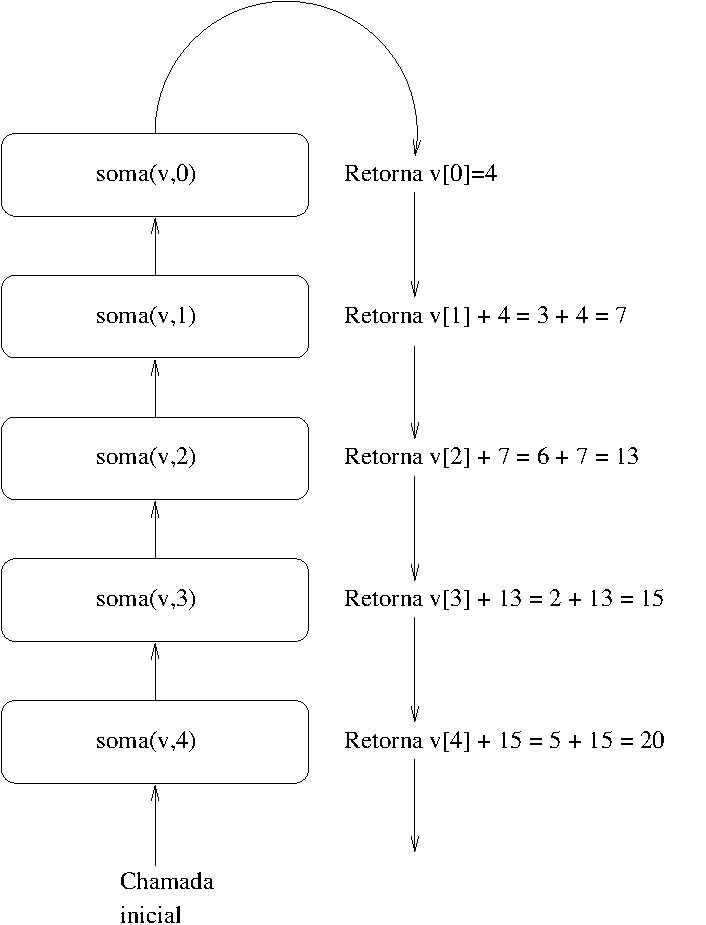
\includegraphics[scale=0.5]{somavetor}
    \end{center}
    \end{minipage}

\end{frame}

%%%%%%%%%%%%%%%%%%%%%%%%%%%%%%%%%%%%%%%%%%%%%%%%%%%%%%%%%%%%%
\begin{frame}[fragile]{Soma de vetor}

    Neste problema, a solução iterativa seria melhor (não há criação de variáveis das chamadas recursivas):
    \begin{minted}{c}
        int calcula_soma(int[] v, int n) {
            int soma = 0, i;
            for (i = 0; i <= n; i++)
                soma = soma + v[i];
            return soma;
        }
    \end{minted}

\end{frame}

%%%%%%%%%%%%%%%%%%%%%%%%%%%%%%%%%%%%%%%%%%%%%%
%%%%%%%%%%%%%%%%%%%%%%%%%%%%%%%%%%%%%%%%%%%%%%
%%%%%%%%%%%%%%%%%%%%%%%%%%%%%%%%%%%%%%%%%%%%%%
%%%%%%%%%%%%%%%%%%%%%%%%%%%%%%%%%%%%%%%%%%%%%%
%%%%%%%%%%%%%%%%%%%%%%%%%%%%%%%%%%%%%%%%%%%%%%
%%%%%%%%%%%%%%%%%%%%%%%%%%%%%%%%%%%%%%%%%%%%%%

\section{Informações extras: biblioteca \texttt{string.h}}

%%%%%%%%%%%%%%%%%%%%%%%%%%%%%%%%%%%%%%%%%%%%%%%
\begin{frame}[fragile]{Biblioteca \texttt{string.h}}

    A função \cod{strcat} faz concatenação de strings.

    Ela recebe duas strings como parâmetro e concatena a string dada no segundo parâmetro no final da string dada no primeiro parâmetro.

    Deve haver espaço suficiente na primeira string, caso contrário ocorrerá um erro.

    \begin{minted}[fontsize=\scriptsize]{c}
        #include <stdio.h>
        #include <string.h>

        int main() {
            char s1[80] = "ola ", s2[80] = "turma de PE!";
            /* concatena s2 no final de s1: */
            strcat(s1, s2);
            printf("%s\n", s1);
            return 0;
        }
    \end{minted}

    A saída será
    \begin{minted}[fontsize=\scriptsize]{bash}
        ola turma de PE!
    \end{minted}

\end{frame}

%%%%%%%%%%%%%%%%%%%%%%%%%%%%%%%%%%%%%%%%%%%%%%%%%%%
\begin{frame}[fragile]{Biblioteca \texttt{string.h}}

    A função \cod{strcmp} compara duas strings. 
    
    Ela recebe duas strings \cod{s1} e \cod{s2} como parâmetro e devolve:
    \begin{itemize}
        \item 0, caso as duas strings sejam iguais.
        \item um valor menor que 0, caso \cod{s1} seja lexicograficamente menor que \cod{s2}.
        \item um valor maior que 0, caso \cod{s1} seja lexicograficamente maior que \cod{s2}.
    \end{itemize}

\end{frame}

%%%%%%%%%%%%%%%%%%%%%%%%%%%%%%%%%%%%%%%%%%%%%%%%%%%
\begin{frame}[fragile]{Biblioteca \texttt{string.h}}

    \begin{minted}[fontsize=\footnotesize]{c}
        #include <stdio.h>
        #include <string.h>

        int main() {
            char s1[80] = "aab", s2[80] = "aac";
            int r;
            r = strcmp(s1, s2);
            if (r < 0)
                printf("%s vem antes que %s\n", s1, s2);
            else if (r > 0)
                printf("%s vem antes que %s\n", s2, s1);
            else
                printf("sao iguais\n");
            return 0;
        }
    \end{minted}

\end{frame}

%%%%%%%%%%%%%%%%%%%%%%%%%%%%%%%%%%%%%%%%%%%%%%%%%%%
\begin{frame}[fragile]{Biblioteca \texttt{string.h}}

    A função \cod{strcpy} faz cópia de strings.

    Ela recebe duas strings como parâmetro e copia a string dada no segundo parâmetro na string dada no primeiro parâmetro.

    \begin{minted}[fontsize=\scriptsize]{c}
        #include <stdio.h>
        #include <string.h>

        int main() {
            char s1[80], s2[80] = "ola pessoal";
            strcpy(s1, s2);
            printf("%s\n", s1);
            return 0;
        }
    \end{minted}

    A saída será
    \begin{minted}[fontsize=\scriptsize]{bash}
        ola pessoal
    \end{minted}

\end{frame}

%%%%%%%%%%%%%%%%%%%%%%%%%%%%%%%%%%%%%%%%%%%%%%%%%%%
\begin{frame}[fragile]{Biblioteca \texttt{string.h}}

    A função \cod{strlen} calcula o tamanho de uma string.
    
    Ela recebe uma string como parâmetro e devolve o número de caracteres na string até o '\textbackslash0'.

    \begin{minted}[fontsize=\scriptsize]{c}
        #include <stdio.h>
        #include <string.h>

        int main() {
            char s1[80] = "ola pessoal";
            int t = strlen(s1);
            printf("%d\n", t);
            return 0;
        }
    \end{minted}

    A saída será
    \begin{minted}[fontsize=\scriptsize]{c}
        11
    \end{minted}

\end{frame}

%%%%%%%%%%%%%%%%%%%%%%%%%%%%%%%%%%%%%%%%%%%%%%%
%%%%%%%%%%%%%%%%%%%%%%%%%%%%%%%%%%%%%%%%%%%%%%%
%%%%%%%%%%%%%%%%%%%%%%%%%%%%%%%%%%%%%%%%%%%%%%%
%%%%%%%%%%%%%%%%%%%%%%%%%%%%%%%%%%%%%%%%%%%%%%%
%%%%%%%%%%%%%%%%%%%%%%%%%%%%%%%%%%%%%%%%%%%%%%%
%%%%%%%%%%%%%%%%%%%%%%%%%%%%%%%%%%%%%%%%%%%%%%%

\section{Informações extras: representação de matrizes por linearização}

%%%%%%%%%%%%%%%%%%%%%%%%%%%%%%%%%%%%%%%%%%%%%%%
\begin{frame}[fragile]{Informações extras: linearização de índices}

    \begin{itemize}
        \item Podemos usar sempre vetores simples para representar matrizes (na prática o compilador faz isto por você).

        \item Ao declarar uma matriz como \cod{int mat[3][4]}, sabemos que serão alocadas 12 posições de memória associadas com a variável \cod{mat}.

        \item Poderíamos simplesmente criar \cod{int mat[12]}, mas perderíamos a simplicidade de uso dos índices em forma de matriz.
        \begin{itemize}
            \item Você não mais poderá escrever \cod{mat[1][3]}, por exemplo.
        \end{itemize}
    \end{itemize}

\end{frame}

%%%%%%%%%%%%%%%%%%%%%%%%%%%%%%%%%%%%%%%%%%%%%%%
\begin{frame}[fragile]{Informações extras: linearização de índices}

    \begin{itemize}
        \item A {\it linearização de índices} é justamente a representação de matrizes usando-se um vetor simples.
        \item Mas devemos ter um padrão para acessar as posições deste vetor como se sua organização fosse na forma de matriz.
    \end{itemize}

\end{frame}

%%%%%%%%%%%%%%%%%%%%%%%%%%%%%%%%%%%%%%%%%%%%%%%
\begin{frame}[fragile]{Informações extras: linearização de índices}

    \begin{itemize}
        \item Considere o exemplo:\\
            \cod{int mat[12]; /* em vez de int mat[3][4] */}
        \item Fazemos a divisão por linhas como segue:
        \begin{itemize}
            \item Primeira linha: \cod{mat[0]} até \cod{mat[3]}
            \item Segunda linha: \cod{mat[4]} até \cod{mat[7]}
            \item Terceira linha: \cod{mat[8]} até \cod{mat[11]}
        \end{itemize}
        \item Para acessar uma posição \cod{[i][j]} usamos:\\
            \cod{mat[i * 4 + j];}\\
            onde $0 \le i \le 2$ e $0 \le j \le 3$.
    \end{itemize}

\end{frame}

%%%%%%%%%%%%%%%%%%%%%%%%%%%%%%%%%%%%%%%%%%%%%%%
\begin{frame}[fragile]{Informações extras: linearização de índices}

    \begin{itemize}
        \item De forma geral, seja matriz \cod{mat[n * m]}, representando \cod{mat[n][m]}.
        \item Para acessar a posição correspondente à \cod{[i][j]} usamos:\\
            \cod{mat[i * m + j];}\\
            onde $0 \le i \le n-1$  e $0 \le j \le m-1$.
        \item Note que $i$ ``pula'' blocos de tamanho $m$, e $j$ indexa a posição dentro de um bloco.
    \end{itemize}

\end{frame}

%%%%%%%%%%%%%%%%%%%%%%%%%%%%%%%%%%%%%%%%%%%%%%%
\begin{frame}[fragile]{Informações extras: linearização de índices}

    \begin{itemize}
        \item Podemos estender para mais dimensões.
        \item Seja matriz \cod{mat[n * m * q]}, representando \cod{mat[n][m][q]}.
        \begin{itemize}
            \item As posições de 0 até $(m * q) - 1$ são da primeira matriz.
            \item As posições de $(m * q)$ até $(2 * m * q) - 1$ são da segunda matriz.
            \item etc\ldots
        \end{itemize}
        \item Para acessar a posição correspondente à $[i][j][k]$ usamos:\\
            \cod{mat[i * m * q + j * q + k];}
    \end{itemize}

\end{frame}

%%%%%%%%%%%%%%%%%%%%%%%%%%%%%%%%%%%%%%%%%%%%%%%
\begin{frame}[fragile]{Informações extras: linearização de índices}

    \begin{minted}[fontsize=\footnotesize]{c}
        int main() {
            int mat[40]; /* representando mat[5][8] */
            int i, j;

            for (i = 0; i < 5; i++)
                for(j = 0; j < 8; j++)
                    mat[i * 8 + j] = i * j;

            for (i = 0; i < 5; i++) {
                for(j = 0; j < 8; j++)
                    printf("%d, ", mat[i * 8 + j]);
                printf("\n");
            }
            return 0;
        }
    \end{minted}

\end{frame}

%%%%%%%%%%%%%%%%%%%%%%%%%%%%%%%%%%%%%%%%%%%%%%
%%%%%%%%%%%%%%%%%%%%%%%%%%%%%%%%%%%%%%%%%%%%%%
%%%%%%%%%%%%%%%%%%%%%%%%%%%%%%%%%%%%%%%%%%%%%%
%%%%%%%%%%%%%%%%%%%%%%%%%%%%%%%%%%%%%%%%%%%%%%
%%%%%%%%%%%%%%%%%%%%%%%%%%%%%%%%%%%%%%%%%%%%%%
%%%%%%%%%%%%%%%%%%%%%%%%%%%%%%%%%%%%%%%%%%%%%%

\section{Exercícios}

%%%%%%%%%%%%%%%%%%%%%%%%%%%%%%%%%%%%%%%%%%%%%%
\begin{frame}[fragile]{\exercicio}

    Escreva um programa que lê 10 números inteiros e os salva em um vetor.
    Em seguida o programa deve encontrar a posição do maior elemento do vetor e imprimir esta posição.

\end{frame}


%%%%%%%%%%%%%%%%%%%%%%%%%%%%%%%%%%%%%%%%%%%%%%
\begin{frame}[fragile]{\exercicio}

    Escreva um programa que lê 10 números ponto flutuante e os salva em um vetor.
    Em seguida o programa deve calcular a média dos valores armazenados no vetor e imprimir este valor.

\end{frame}

%%%%%%%%%%%%%%%%%%%%%%%%%%%%%%%%%%%%%%%%%%%%%%
\begin{frame}[fragile]{\exercicio}

    Escreva um programa que lê 10 números inteiros e os salva em um vetor.
    Em seguida o programa deve ler um outro número inteiro $C$.
    O programa deve então encontrar dois números em posições distintas do vetor cuja multiplicação seja $C$ e imprimí-los.
    Caso não existam tais números, o programa deve informar isto.

    \textbf{Exemplo}: Se $vetor = (2, 4, 5, -10, 7)$ e $C=35$, então o programa deve imprimir ``5 e 7''.
    Se $C=-1$, então o programa deve imprimir ``Não existem tais números''.

\end{frame}

%%%%%%%%%%%%%%%%%%%%%%%%%%%%%%%%%%%%%%%%%%%%%%%%%%%
\begin{frame}[fragile]{\exercicio}

    Escreva um programa que lê uma string de até 50 caracteres, e imprime ``Palindromo'' caso a string seja um palindromo e ``Nao Palindromo'' caso contrário.

    Obs.: Um palíndromo é uma palavra ou frase que é igual quando lida da esquerda para a direita ou da direita para a esquerda (espaços em brancos são descartados).
    
    Assuma que as palavras são todas escritas em letras minúsculas e sem acentos.

    Exemplo de palíndromo: "saudavel leva duas".

\end{frame}

%%%%%%%%%%%%%%%%%%%%%%%%%%%%%%%%%%%%%%%%%%%%%%%%%%%
\begin{frame}[fragile]{\exercicio}

    Refaça o exemplo visto em aula de inversão de uma string de tal forma que não seja utilizado nenhum vetor adicional!

    Isto é, devemos computar a inversa no próprio vetor onde a string foi lida.

\end{frame}

%%%%%%%%%%%%%%%%%%%%%%%%%%%%%%%%%%%%%%%%%%%%%%
\begin{frame}[fragile]{\exercicio}
    
    Faça um programa para realizar operações com matrizes que tenha as seguintes funcionalidades:
    \begin{itemize}
        \item Um menu para escolher a operação a ser realizada:
        \begin{enumerate}
            \item Leitura de uma matriz $M_1$.
            \item Leitura de uma matriz $M_2$.
            \item Impressão das matrizes $M_1$ e $M_2$.
            \item Impressão da soma de $M_1$ com $M_2$.
            \item Impressão da multiplicação de $M_1$ com $M_2$.
            \item Impressão da subtração de $M_2$ de $M_1$.
            \item Impressão da transposta de $M_1$ e $M_2$.
        \end{enumerate}
    \end{itemize}

\end{frame}

%%%%%%%%%%%%%%%%%%%%%%%%%%%%%%%%%%%%%%%%%%%%%%%
\begin{frame}[fragile]{\exercicio}

    Escreva um programa que leia todas as posições de uma matriz $10 \times 10$.
    
    O programa deve então exibir o número de posições não nulas na matriz.

\end{frame}

%%%%%%%%%%%%%%%%%%%%%%%%%%%%%%%%%%%%%%%%%%%%%%%
\begin{frame}[fragile]{\exercicio}

    Escreva um programa que lê todos os elementos de uma matriz $4 \times 4$ e mostra a matriz e a sua transposta na tela.

    \begin{center}
    \begin{tabular}{c c}
        Matriz & Transposta \\
        $\left[\begin{array}{c c c c}
            0 & 1 & 0 & 2 \\
            0 & 1 & 0 & 2 \\
            0 & 1 & 0 & 2 \\
            0 & 1 & 0 & 2 \\
        \end{array}\right]$ &

        $\left[\begin{array}{c c c c}
            0 & 0 & 0 & 0 \\
            1 & 1 & 1 & 1 \\
            0 & 0 & 0 & 0 \\
            2 & 2 & 2 & 2 \\
        \end{array}\right]$
    \end{tabular}
    \end{center}

\end{frame}

%%%%%%%%%%%%%%%%%%%%%%%%%%%%%%%%%%%%%%%%%%%%%%%
\begin{frame}[fragile]{\exercicio}

    Escreva um programa que lê uma matriz do teclado e então imprime os elementos com menor e maior frequência de ocorrência na matriz.

\end{frame}

%%%%%%%%%%%%%%%%%%%%%%%%%%%%%%%%%%%%%%%%%%%%%%%%%%%%%%%%%%%%%%
\begin{frame}[fragile]{\exercicio}

    Escreva um algoritmo iterativo que, dado um inteiro $n$ e um vetor de inteiros $v$ de tamanho $t$, devolve um inteiro $i$ tal que $v[i] == n$ ou $-1$ caso $n$ não esteja presente em $v$.

    Reescreva o algoritmo acima de maneira recursiva.

\end{frame}

%%%%%%%%%%%%%%%%%%%%%%%%%%%%%%%%%%%%%%%%%%%%%%%%%%%%%%%%%%%%%%
\begin{frame}[fragile]{\exercicio}

    Escreva um programa que lê uma palavra do teclado e então imprime todas as permutações desta palavra.

    Se por exemplo for digitado ``abca'' o seu programa deveria imprimir:

    \begin{minted}[fontsize=\scriptsize]{bash}
        aabc
        aacb
        abac
        abca
        acab
        acba
        baac
        baca
        bcaa
        caab
        caba
        cbaa
    \end{minted}

\end{frame}

%%%%%%%%%%%%%%%%%%%%%%%%%%%%%%%%%%%%%%%%%%%%%%%%%%%%%%%%%%%%%
\begin{frame}[fragile]{\exercicio}

    Mostre a execução da função \cod{imprime}. O que será impresso?

    \begin{minted}[fontsize=\scriptsize]{c}
        #include <stdio.h>

        void imprime(int v[], int i, int n);

        int main() {
            int vet[] = {1, 2, 3, 4, 5, 6, 7, 8, 9, 10};
            imprime(vet, 0, 9);
            printf("\n");
            return 0;
        }
        void imprime(int v[], int i, int n) {
            if (i == n) {
                printf("%d, ", v[i]);
            } else {
                imprime(v, i+1, n);
                printf("%d, ", v[i]);
            }
        }
    \end{minted}
\end{frame}

\end{document}
